\documentclass{article}

\title{ProjectProposal}
\author{Adrian Alberdi \\and \\Leonard Eschenbaum}
\date{}

\usepackage{graphicx}
\begin{document}
\maketitle

\section{Enterprise Description}
\paragraph{Name:} Smoking Games

\paragraph{Description:} Smoking games it's an enterprise that digitally distributes games, created by themselfs or third party games.
\section{Enterprise structure}
	The enterprise has the following structure:

\begin{figure}[htp] \centering
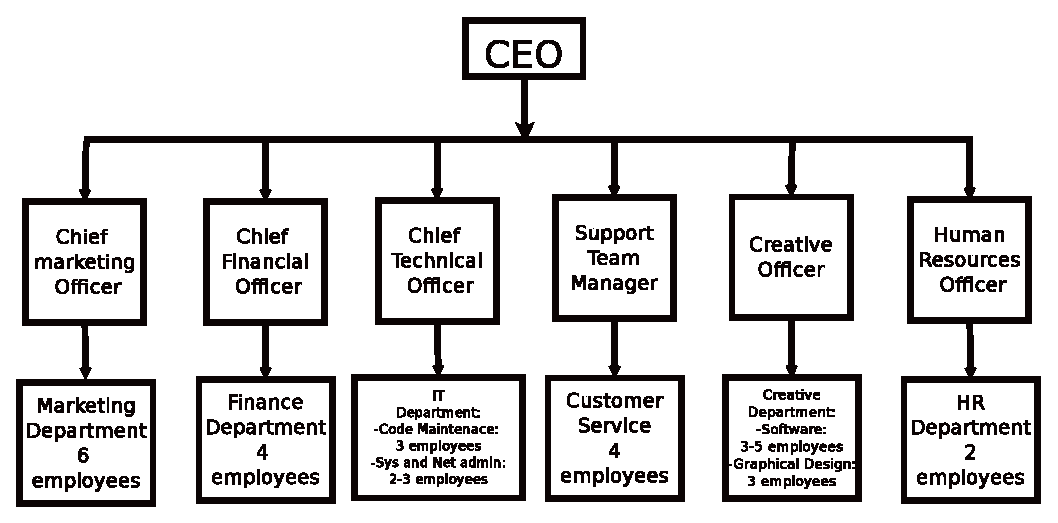
\includegraphics[scale=0.8]{Organizational_hierarchy.eps}
\caption{How the enterprise works}
\label{}
\end{figure}

Total number of workers: 33-36 people

\section{References:}

Michael E. Whitman and Herbert J.Mattford. \emph{Principles of Incident Response and Disaster
Recovery}

Business and IT Continuity: Overview and Implementation Principles is a deliverable by the European Union Network and Information Security Agency (ENISA) that elaborates on continuity risks and contains an overview of numerous Business Continuity models
\end{document}